\documentclass[]{report}

\usepackage{amsmath}
\usepackage{graphicx}
\usepackage{algorithm}
\usepackage{hyperref}       % hyperlinks
\usepackage{url}            % simple URL typesetting
\usepackage{booktabs}       % professional-quality tables
\usepackage{amsfonts}       % blackboard math symbols
\usepackage{nicefrac}       % compact symbols for 1/2, etc.
\usepackage{microtype}      % microtypography
\usepackage{amssymb}
\usepackage{amsmath}
\usepackage[utf8]{inputenc}
\usepackage[english]{babel}
\usepackage{tikz}
%\usepackage{subfigure}
%%\usepackage{tikz}
%\usepackage{algorithm}
\usepackage{algpseudocode}
\usepackage{chngcntr}
%\usepackage{graphicx}
%\usepackage{subfig}
\newcommand{\tif}{\textit}
\newcommand{\tbf}{\textbf}
\renewcommand{\thesection}{\arabic{section}}
% Title Page
\title{Hamiltonian Monte Carlo}
\author{Bradley Gram-Hansen}


\begin{document}
\maketitle


\section{Intro to HMC MCMC}

Following Neal 2011 Chapter 5 Handbook of MCMCM
\subsection{Metropolis-hastings algorithm}
The Metropolis hastings algorithm is the work horse of Monte Carlo Markov Chain (MCMC) methods, It relies on a simple reject and accept criteria for determining whether or not we should proceed to some next state. If our state is accepted, but does not satisfy the full criteria then a probability is associated with that state, and if that probability exceeds the one sampled from a given cut off, usually determined by sampling from a uniform distribution then it is accepted, else rejected. 

\begin{algorithm}
\caption{Metropolis-Hasting algorithm}
\begin{algorithmic}[1]
	\State  $x^{0} \sim P_{0}(x)$ \Comment{Where $p(x)$ is the proposed initial distribution}
	\For {$i = 0,1,2,\ldots$}
	\State $ x \gets x^{s} $
	\State $ x^{'} \sim Q(x^{'}|x)$
	\State $a = \frac{\tilde{P}(x')Q(x|x')}{\tilde{P}(x)Q(x'|x)}$ \Comment{Acceptance ratio}
	\State $r = min(1, a) $ \Comment{Acceptance condition}
	\State $u \sim  U(0,1)$ 
	\State $x^{i+1} = \begin{cases}
	x' \text{ if $u < r$}\\
	x^{i} \text{ if $u \geq r$}
	\end{cases}$
	\EndFor
	\State \Return $x^{i+1}$
\end{algorithmic} 
\end{algorithm}

\subsection{HMC for MCMC}

In a top level view Hamilton Monte Carlo for Monte Carlo Markov Chain (HMC MCMC) is a two step process. In step one we define a Hamiltonian function in terms of the probability distribution from which we wish to sample from. We introduce a position variable, $q$ and momentum variable $p$, where $p$ is an auxiliary variable that typically has a Gaussian distribution.  All $p$'s are assumed independent. 
In step two, the HMC alternates simple updates for the momentum variables with Metropolis updates. This enables us to propose a new state by computing a trajectory according to Hamiltonian dynamics, implemented with the leapfrog method. 
\subsubsection{Prerequisites}
The Hamiltonian of a physical system is defined completely with respect to the position $q$ and $p$ momentum variables, which span the phase space of the system. The Hamiltonian is the Legendre transform of the Lagrangian and gives us the total energy in the system. It is defined as follows: 
\begin{equation}
\label{eq:hamiltonian}
 H(\textbf{q},\textbf{p}) = \sum_{i = 1}^{d}\dot{q}_{l}p_{l} - L(\textbf{q}, \textbf{\.{q}}(\textbf{q}, \textbf{p}))
\end{equation}
where $d$ is the system dimensions, and so the full state space with has $2d$ dimensions.  
Thus, for simplicity, if we set $d = 1$ we can derive the Hamiltonian equations as follows:\begin{equation}
\label{eq:hameq1}
\frac{\partial H}{\partial p} = \dot{q} + p\frac{\partial \dot{q}}{\partial p} - \frac{\partial L}{\partial \dot{q}}\frac{\partial \dot{q}}{\partial p} = \dot{q} \end{equation}
and 
\begin{equation}
\label{eq:hameq2}
\frac{\partial H}{\partial q} = p\frac{\partial \dot{q}}{\partial q} - \frac{\partial L}{\partial q} - \frac{\partial L}{\partial \dot{q}}\frac{\partial \dot{q}}{\partial q} = - \frac{\partial L}{\partial q}= -\dot{p}  \end{equation}
and the process is the same for more than one dimension. 
We can write \ref{eq:hamiltonian}\ more succinctly as:
\begin{equation}
\label{eq:hamreduced}
H(\textbf{q}, \textbf{p})  = K(p) + U(q)
\end{equation}
where $K(p)$ represents our kinetic energy and $U(q)$ is the potential energy.

Within the HMC MCMC framework the ''positions", $q$, are the variables of interest and for each position variable we have to create a fictitious ''momentum", $p$. For compactness let $z = (q,p)$. The potential energy $U(q)$ will be the minus of the log of the probabilty density for the distribution of the position variables we wish to sample, plus \textbf{any} constant that is convenient.  The kinetic energy will represents the dynamics of our variables, for which a popular form of $K(p) = \frac{p^{T} M^{-1} p}{2}$, where $M$ is symmetric, positive definite and typically diagonal. This form of $K(p)$ corresponds to a minus the log probability of the zero mean Gaussian distribution with covariance matrix $M$. For this choice we can write the Hamiltonian equations, for any dimension $d$, as follows:
\begin{align}
\dot{q}_{i} &= \frac{dq_{i}}{dt} = [M^{-1}p]_{i} \\
\dot{p}_{i} &= \frac{dp_{i}}{dt} = -\frac{\partial U}{\partial q_{i}}
\end{align}

To view the Hamiltonian in terms of probabilities, we use the concept of the canonical distribution from Statistical mechanics to construct our pdf. Thus, the distribution that we wish to sample from can be related to the potential energy via the canonical distribution as:
\begin{equation}
\label{eq:canonical}
P(z) = \frac{1}{Z}\exp\left(\frac{-E(z)}{T}\right)
\end{equation}
As the Hamiltonian is just an energy function we may can insert \ref{eq:hamreduced}\ into our canonical distribution \ref{eq:canonical}\, which gives us the joint density:
\begin{equation}
P(q,p) = \frac{1}{Z}\exp(-U(q))\exp(-K(p)  
\end{equation}
where $T = 1$ is fixed. And so we can now very easily get to our target distribution $p(q)$, which is dependent on our choice of potential $U(q)$, as this expression factorizes in to two independent probability distributions. 
We characterise the posterior distribution for the model parameters using the potential energy function: \begin{equation}
U(q) = -\log[\pi(q)L(q|D)]
\end{equation}
where $\pi(q)$ is the prior distribution, and $L(q|D)$ is the likelihood, not the Lagrangian, of the given data $D$. 

\subsection{The Integrator}

\subsubsection{The leapfrog method}
The leapfrog method enables reduced error and allows us to dicretize Hamiltons equations, so that we can implement them numerically. 
We start with a state at $t = 0$ and then evaluate at a subsequent time $t + \epsilon , \hdots, t + n\epsilon$, where $\epsilon$ is the step in which we increase and $n$ is the number of time steps. 

\begin{align}
p_{i}(t + \frac{\epsilon}{2}) &= p_{i}(t) - \left(\frac{\epsilon}{2}\right)\frac{\partial U(q(t))}{\partial q_{i}} \\
q_{i}(t + \epsilon) &= q_{i}(t) + \epsilon\frac{\partial K(p(t + \frac{\epsilon}{2}))}{dp_{i}}\\
p_{i}(t + \epsilon) &= p_{i}(t + \frac{\epsilon}{2}) - \left(\frac{\epsilon}{2}\right)\frac{\partial U}{\partial q_{i}}\\
\end{align}
\footnote{For the usual choice of kinetic energy, we have $\frac{\partial K(p + \frac{\epsilon}{2})}{dp_{i}} = \frac{p_{i}(t + \frac{\epsilon}{2})}{m_{i}}$}

For the leapfrog method the local error, error after one step, is of $\mathcal{O}(\epsilon^{2})$ and a global error, error after simulating for some fixed time interval s, which requires $\frac{s}{\epsilon}$ is $\mathcal{O}(\epsilon^{3})$
\subsubsection{Some initial points of notice}
Neals implementation of the HMC can only be used to sample from continuous distributions on $\mathbb{R}^{d}$ for which a density function can be evaluated.\\
We must be able to compute the partial derivative of the log of the density function. The derivaties must exists at the points at which they are evaluated [\textbf{Automatic differentiation}]

HMC samples from the canonical distribution for $q$ and $p$. $q$ has the distribution of interest as specified by the potential $U(q)$. 
The distribution of the $p$'s can be chosen by us and are independent of the $q$'s. 
The $p$ components are specified to be independent, with component $p_{i}$ having variance $m_{i}$.
The kinetic energy $K(p) = \sum_{i =1}^{d}\frac{p_{i}^{2}}{2m_{i}}(q(t + \epsilon))
$

\subsubsection{The steps}

\begin{enumerate}
	\item Step 1: Changes only the momentum
	\item Step 2: May change both position and momentum
\end{enumerate}
Both steps leave the canonical distribution of (q,p) invariant, hence the distribution remains invariant.

In \textbf{Step 1} we first draw the $p_{i}$ randomly from their Gaussian distribution independently of the current values of the position values. 
In \textbf{Step 2} a Metropolis update is performed, using the Hamiltonian dynamics to propose a new state. Starting with the current state $(q,p)$, Hamiltonian dynamics is simulated for $L$ steps using the leapfrog method, with a stepsize of $\epsilon$. $L$ and $\epsilon$ are parameters of the mnodel that need to be tuned.\\
The momentum vairables at the end of this $L$-step trajectory are then negated, giving s proposed state $(q^{*}. p^{*})$. This proposed state is accepted as the next state in the Markov Chain with probability: \begin{equation}
\min[1, \exp(-H(q^{*}, p^{*}) + H(p,q)] = \min[1, \exp(-U(q^{*}) + U(q) - K(p^{*}) + K(p))]
\end{equation} 
\begin{algorithm}
	\label{alg:simpHMC}
	\caption{\textbf{Continuous Hamiltonian Monte Carlo MCMC}}
		\begin{algorithmic}[1]
			\Procedure{HMC}{$\theta_{0}$, $\epsilon$, $L$,$U$, $M$}
			\For{$m = 1 \text{ to } M$}
			\State $ p^{0} \sim \mathcal{N}(0,\mathbb{I})$
			\State $ \theta^{m} \gets \theta^{m-1}$
			\State $\theta^{'} \gets \theta^{m-1}$
			\State $ p^{'} \gets p^{0}$
			\For {$i = 1 \text{ to } L$}
			\State $\theta^{'}$ , $p \gets$ Leapfrog($\theta^{'}, p^{'}, \epsilon$)
			\EndFor
			\State $\alpha = \min\left\{1, \frac{\exp \left\{-U(\theta^{'}) - K(p^{'})\right\}}{\exp \left\{U(\theta^{m-1}) - K(p^{0})\right\}}\right\}$ \Comment{Acceptance probability}
			\State $u \sim Uniform(0,1)$
			\If{ $u < \alpha $}
			\State \Return $ \theta^{m} \gets \theta^{'}$, $p^{m} \gets -p $  \Comment{Accept}
			\Else
			\State \Return $\theta^{m}  \gets \theta^{m-1}$ , $p^{m} \gets p^{0}$ \Comment{Reject}
			\EndIf
			\EndFor
			\State {Leapfrog($\theta$, $p$, $\epsilon$)} 
			\State $p^{'} \gets p - \frac{\epsilon}{2}\nabla_{\theta} U(\theta)$ \Comment{Half step for momentum}
			\State $\theta^{'} \gets \theta + \epsilon \nabla_{p} K(p^{'})$ \Comment{Full step for the the position} 
			\State $p^{'} \gets \frac{\epsilon}{2}\nabla_{\theta}U(\theta^{'})$ \Comment{Final half step for momentum}
			\State \Return $\theta^{'}$ , $p^{'}$
	\end{algorithmic} 
\end{algorithm}
If the proposed state is rejected, then the next state is the same as the current state and is counted again when calculating the expected value of some function. 
The negation of the momentum variables at the end of the trajectory makes the Metropolis proposal symmetrical, as needed for the acceptance probability above to be valid. This negation need not be done in practice, since $K(p) = K(-p)$, and the momentum will be replaced before it is used again, in the first step of the next iteration.
Where $U = -\log(\pi(\theta))$,  $M$ is the number of samples we wish to take , $(\theta^{'}, p^{'})$ is the generated proposal and we propose setting $\theta^{m} = \theta^{'}$ and $p^{m} = -p^{'}$ and then accept or reject this proposal according to the Metropolis update step. 
A function that implements a single iteration of the HMC algorithm is given in algorithm 2. There are three additional functions within this iteration: $U$, which returns the potential energy given a value for $q$,  $\nabla U$, which returns the vector of partial derivatives of $U$ given $q$ and $\nabla K$, which returns the vector of partial derivatives of $K$ given $p$. Other arguments are the stepsize, $\epsilon$, for leapfrog steps, the number of leapfrog steps in the trajectory, $L$, and the current position, $q_{current}$, that the trajectory starts from. Momentum variables are sampled within this function, and discarded at the end, with only the next position being returned. 

\section{Discrete 'Discontinuous' Hamiltonian Monte Carlo (DHMC)}

Heavily Based on the paper by Nishimura et al. 2017. \\
\textbf{Note: } $q \rightarrow \theta$
The DHMC can handle discontinuous posterior distributions. 
\\
\textbf{Key Ideas:}
\begin{itemize}
	\item Embedding of discrete parameters into a continous space, inducing parameters with piecewise constant densities. 
	\item Simulation of Hamiltonian dynamics on a piecewise smooth density function
\end{itemize} 
Given any target distribution, for each iteration, DHMC only requires evaluations of the density and the following:
\begin{itemize}
	\item The full conditional densities of the discrete parameters up to a normalising constant. 
	\item Which is done via evaluations of a directed acryclic graph framework, taking advantage of conditional independence structure (Lunn et al 2009)
	\item Either the gradient of the log density w.r.t. continuous parameters or their individual full conditional densities. 
\end{itemize}

\subsection{Embedding Discrete Parameters Into a Continuous Space}

Let $N$ denote a discrete parameter with prior distribution $\pi_{n}(\cdot)$, assume with out loss of generality that $N \in \mathbb{N}$. To embed $N$ into a continuous space, we introduce
a latent parameter $\tilde{N}$, whose relationship with $N$ is defined as follows: $N = n \iff \tilde{N}\in(a_{n}, a_{n+1}] $ for a sequence $0 = a_{1} \leq a_{2} \leq \ldots$, where $a_{n} \in \mathbb{R}$. \\
\begin{figure}[h!]
	\centering
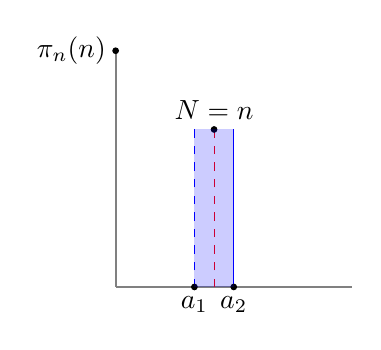
\begin{tikzpicture}
\draw[gray, thick] (0,0) -- (0,3);
\draw[gray, thick] (0,0) -- (3,0);
\draw[red, dashed] (1.25,0) -- (1.25,2);
\draw[blue, dashed] (1,0) -- (1,2);
\draw[blue] (1.5,0) -- (1.5,2);
\filldraw[black](0,3) circle (1pt) node[left] {$\pi_{n}(n)$};
\filldraw[black](1,0) circle (1pt) node[below] {$a_{1}$};
\filldraw[black](1.5,0) circle (1pt) node[below] {$a_{2}$};
\filldraw[black](1.25,2) circle (1pt) node[above] {$N = n$};
\fill[blue, opacity=0.2] (1,0) rectangle (1.5,2);
\end{tikzpicture}
\caption{A view of our continuous embedding of a discrete parameter. The shaded region represents the piecewise constant prior density $\pi_{\tilde{N}}(\tilde{n})$ over $\tilde{N}$}\label{fig:contembedding}
\end{figure}
To match the prior distribution $\pi(N)$, the corresponding, piecewise constant, prior over the latent parameter $\tilde{N}$ is given by: \begin{equation}
\pi_{\tilde{N}}(\tilde{n}) = \sum_{n \geq 1} \frac{\pi_{N}(n)}{a_{n+1} - a_{n}} \mathbb{I}(a_{n} < \tilde{n} \leq a_{n+1}) 
\end{equation}
where the Jacobian-like factor $(a_{n+1} - a_{n})^{-1}$ adjusts for embedding into non-uniform intervals. Rather than pick uniform embedding such as $a_{n} = n$ for all $n$, it is better to use a non-uniform one. For example $a_{n} = log(a_{n})$.

\subsubsection{Why does the HMC fail for discrete parameters}
When the target distribution $\pi_{\theta}(\cdot)$ has discrete parameters, we have discontinuities. Thus, when we try and perform our integrator step incorporating Hamiltonian dynamics, 
which will depend on derivatives that require continuity, we of course are going to fail.

\subsection{Resolution}
To resolve this at points of discontinuity we need a correct limiting procedure to take into account the steps. A note on integrability, provided the discontinuities at the boundaries can be detected, Hamiltonians equations can be integrated to take into account the instantaneous change in $pi_{\theta}(\cdot)$ . We do this by constructing a discontinuous set from $U(\Theta) = -log_{\pi(\theta)}(\theta)$, the potential energy, to form a piecewise smooth manifold.\\

Whilst it is true that a discontinuous function does not have a \tif{well defined} derivative in the classical sense, the gradient of the potential can be defined through a distributional derivative, which allows us to interpret Hamiltonians equations \ref{eq:hameq1}\ \ref{eq:hameq2} as a measure-valued differential equation. There is however a cravat, that being the solution to a measure-value differential equation is not unique. To circumvent this we use the \textbf{selection principle} (Ambrosio 2008) and construct a solution with desirable properties.
In general, the process is as follows: Define a sequence of smooth approximations $U_{\delta}(\theta)$ of $U(\theta)$, for $\delta > 0$. We construct the smooth approximations through a convolution $U_{\delta} = U \ast \phi_{\delta}$, with $\phi_{\delta}(\theta) = \delta^{-d}\phi(\delta^{-1}\theta)$. Where $\phi$ is a compactly smooth function, i.e a function that has all the required properties to be a probability distribution $\phi \ge 0$ s.t. $\int \phi = 1$ and $d$ is the dimension of $\theta$.

\subsection{Defining the trajectory}
Let $\theta_{\delta}(t), p_{\delta}(t)$ be a solution to Hamilton's equations, with potential energy $U_{\delta}$. Taking the limit as $\delta \rightarrow 0$ leads to the true trajectory $(\theta(t), p(t))$. Although the limit exists for most trajectories, it does exist for all (proof?). Despite this we define the dynamics of $U(\theta)$ in terms of this point wise limit. 
Suppose the trajectory $(\theta(t), p(t))$ hits the discontinuity at an event time $t_{e}$. Let $t_{e_{-}}$ and $t_{e_{+}}$ denote the infinitesimal moment before and after that point, i.e our limiting values.\\
Since the discontinuity set of $U(\theta)$ was assumed to be piecewise smooth, at a discontinuity point $\theta$ we have:
\begin{equation}
\label{eq:discpoint}
 \lim_{\delta \to 0} \frac{\nabla_{\theta} U_{\delta}(\theta)}{||\nabla_{\theta}U_{\delta}(\theta)||}=\nu(\theta) 
\end{equation}   

where $\nu(\theta)$ denotes a unit vector orthonormal to the discontinuity, pointing in the direction of the higher potential. The relation \ref{eq:discpoint}\ and $\frac{dp_{\sigma}}{dt} = -\nabla_{\theta}U_{\delta}$ imply that the only change in $p(t)$ upon encountering the discontinuity occurs in the direction of $\nu_{e} = \nu(\theta(t_{e}))$, that being:\begin{equation}
p(t_{e_{+}}) = p(t_{e_{-}}) - \gamma \nu_{e}
\end{equation}
for some $\gamma > 0$. There are two types possible types of change in $p$ depending on the potential energy difference $\nabla U_{e}$ at the discontinuity, which are defined formally as: \begin{equation}
\nabla U_{e} = \lim_{\epsilon \to 0^{+}} U(\theta(t_{e})) + \epsilon p(t_{e_{-}}) - U(\theta(t_{e_{}}))
\end{equation} 
when the momentum does not provide enough kinetic energy to overcome the potential energy increase $\nabla U_{e}$, the trajectory bounces back against the plane orthogonal to $\nu_{e}$, see figure \ref{fig:bounceback}\ . Else, the trajectory, particle, moves through the potential by transferring kinetic energy to potential energy.
The magnitude of the instantaneous change $\gamma$ is determined by looking at the conversation of energy: \begin{equation}
K(p(t_{e_{+}})) - K(p(t_{e_{-}})) = U(\theta(t_{e_{-}})) - U(\theta(t_{e_{+}}))
\end{equation}
\begin{figure}
	\centering
	\label{fig:bounceback}
		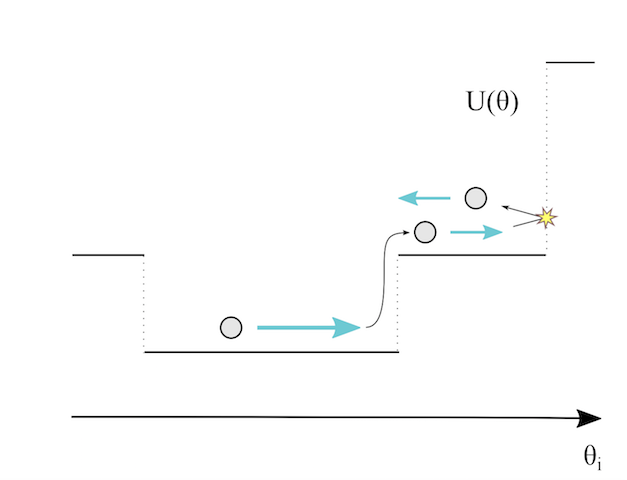
\includegraphics[\textwidth]{bounceback.png}
	\caption{If there is not enough momentum energy, then the particle cannot progress to the step}
\end{figure}


\subsection{The need for a new momentum}
In the discrete setting Gaussian momentum defined in the Kinetic energy, $K(p) = \frac{p\cdot p}{m}$ does not work efficiently, as we now need to perform additional computations to detect the discontinuities. This leads [Nishimura et al. 2017] to use independent Laplace momentums, drawn from a Laplace distribution $\pi_{p}(p) \propto \Pi_{i} \exp(-\frac{|p_{i}|}{m_{i}})$. This allows us to construct a reversible integrator that can jump through multiple discontinuities in a small number of target density evaluations, while preserving the total energy. 
Under the Laplace momentum Hamiltonians equations become: \begin{align}
\label{eq:hamlaplace1}
\dot{\theta} &= m^{-1} \odot \text{sign}(p)\\
\label{eq:hamlaplace2}
\dot{p} &= -\nabla_{\theta} U(\theta)
\end{align}
and so we only depend on the sign of $p$ and not the magnitudes. If we know that $p_{i}(t)$'s do not change their signs on the time interval $t \in [\tau, \tau + \epsilon]$, then we also know that the full step for the position will be:\begin{equation}
\theta(t + \epsilon) = \theta(\tau) + \epsilon m^{-1} \odot \text{sign}(p(\tau))
\end{equation} irrespective of the intermediate values $U(\theta(t))$ along the trajectory $(\theta(t),p(t))$ for $t \in [\tau, \tau + \epsilon]$. The ability of the integrator to jump through multiple discontinuities of $U(\theta)$ in a single target density evaluation depends critically on $\theta(\tau + \frac{\epsilon}{2})$. Where as the momentum step $p(\tau + \epsilon)$ is dependent on the intermediate values $U(\theta(t))$. This can actually be solved by splitting the differential operator in \ref{eq:hamlaplace2}\, into its coordinate-wise component. 
\subsection{Creating an Integrator for Laplace Momentum via Operator Splitting}

To derive a scheme for the integrator under a independent Laplace momentum, we consider the equation for each coordinate $(\theta_{i}, p_{i})$, while the other parameters $(\theta_{-i},p_{-i})$ are fixed, which would mean that the only non-zero derivatives are given by:\begin{equation}
	\dot{\theta_{i}} = m^{-1}_{i} \text{sign}(p_{i}), \hspace{2mm} \dot{p_{i}} = -\nabla_{\theta_{i}} U(\theta) 
\end{equation}
In the case that the initial momentum is large enough that $m^{-1}_{i}|p_{i}(\tau)| > U(\theta^{*}(t)) - U(\theta(\tau))$ for all $t \in [\tau, \tau + \epsilon]$, we have: \begin{equation}
	\theta(t + \epsilon) = \theta^{*}(\tau + \epsilon) + \epsilon m^{-1} \odot \text{sign}(p(\tau))
\end{equation}

Otherwise, the momentum is $p_{i}$ flips, and the trajectory $\theta(t)$ reverses its course at the event time $t_{e}$, figure \ref{fig:bounceback}\,  given by:\begin{equation}
	t_{e} = \inf\{t \in [\tau. \tau + \epsilon] : U(\theta^{*}(t)) - U(\theta(\tau)) > K(p(\tau))\}
\end{equation}
The reversibility of the described integrator is guaranteed by randomly permuting the order of the coordinate updates.\\

\begin{algorithm}
	\label{alg:intcord}
	\caption{Integrator step for purely discrete parameters, with Laplace momentum}
		\begin{algorithmic}[1]
			\Procedure{Cordinate-wise integrator}{$\theta, p, i, \epsilon$}
			\State $ \theta_{i}^{*} \gets \theta$
			\State $ \theta_{i}^{*} \gets \theta^{*}_{i} + \epsilon m^{-1}_{i} \text{sign}(p_{i})$
			\State $ \nabla U \gets U(\theta^{*}) - U(\theta)$
			\If{$m^{-1}_{i}|p_{i}| > \nabla U$}
			\State $ \theta \gets \theta^{*} $
			\State $ p_{i} \gets p_{i} - m_{i} \nabla U$
			\Else
			\State $p_{i} \gets - p_{i}$
			\Endif 
			\State \Return $\theta, p$
		\end{algorithmic} 
\end{algorithm}
Note: To ensure ergodicity we can do as Neal (2010) suggests for the standard HMC by drawing the stepsize from a uniform distribution, where the bounds are the maximum and minimum stepsize, $\epsilon \sim \text{Uniform}(\epsilon_{min}, \epsilon_{max})$. 

\subsection{Mixing Continuous and Discrete Parameters }
Algorithm \ref{alg:intcord} [Should be algo 3] would be valid regardless of whether we are dealing with a discrete or continuous parameter space. However, to increase efficiency and create a faster alogorithm, we can take advantage of the fact that the discontinuities of $U(\theta)$ only occur at a finite number of locations in the trajectory $\theta_{j}$, described via the discontinuity set $\mathcal{D}$, where each discontinuity is indexed by the set $\text{J} = \{j = 1,\ldots,d\} \notin \text{I}$.  Whereas the continuity set, where the trajectory $\theta_{i}$ will be smooth and so to the potential, can be indexed by the set $\text{I} = \{i = 1,\ldots, d\}$. For this system the corresponding kinetic energy is given by: \begin{equation}
K(p) = \frac{1}{2} p_{I}^{T}M_{I}^{-1}p_{I} + \sum_{j \in J}m_{j}^{-1} |p_{j}|
\end{equation}
 where $M_{I}$ and $M_{J} = diag(m_{j})$ are mass matrices.  In constructing the new integrator we first update the smooth parameter $(\theta_{I}, p_{I})$ , second we update the discontinuous parameters $(\theta_{J}, p_{J})$ via algorithm ~\ref{alg:intcord} and finally update $(\theta_{I},p_{I})$.  Where we update $(\theta_{I}, p_{I})$ via the usual leap frog method.  The more efficient integrator is shown in algorithm ~\ref{alg:intforDHMC}.
 
\begin{algorithm}
	\label{alg:intforDHMC}
	\caption{Integrator for discontinuous HMC}
	\begin{algorithmic}[1]
		\Procedure{DHMC full integrator}{$\theta, p, \epsilon, \phi = Permute(J)$}
		\State $ p_{I} \gets p_{I} + \frac{\epsilon}{2}\nabla_{\theta}\log(\pi(\theta_{I}))$
		\State $ \theta_{I} \gets \theta_{I} + \frac{\epsilon}{2} M^{-1}_{I} p_{I}$ \Comment{As I is the continuous set, the momentum here could be Gaussian}
		\For{$j \text{   in   } J$}
		\State $\theta , p \gets \text{Cordinate-wise integrator}(\theta,p,\phi(j), \epsilon)$ 
		\EndFor
		\State $\theta_{I} \gets \theta_{I} + \frac{\epsilon}{2}M_{I}^{-1}p_{I}$
		\State $p_{I} \gets p_{I} + \frac{\epsilon}{2}\nabla_{\theta_{I}}\log(\pi(\theta))$
		\State \Return $\theta, p$ 
		\end{algorithmic} 
\end{algorithm}
\subsubsection{The Role of the mass matrix and stepsize}
As in (Neal 2010) for the standard HMC, if we use a non-identity mass matrix $M$, then that has the effect of reconditioning the target distribution through reparameterization. In general, it is expected that the sampling is facilitated by a reparametrization $\theta_{J} \rightarrow \Lambda_{J}^{-\frac{1}{2}}$ for $\Lambda_{J}  = diag(var(\theta_{J}))$, thus the mass in the momentum distribution is approximately $m_{i} \approx \text{var}(\theta_{j})^{\frac{1}{2}}$. This is also directly related to the step size $\epsilon$, as we increment the parameter $\theta_{j}$ by $\pm \epsilon m_{j}^{-1}$. The problem with this is that it is possible that the if condition in Algorithm \ref{alg:intcord}\ [Should say algo 3] is never satisfied, and so we continually flip the momentum, without ever updating $\theta_{j}$. This will only update when \begin{equation}
\label{eq:condforeps}
	U(\theta + \epsilon m_{j}^{-1} \text{sign}(p_{j}) e_{j})  -U(\theta) < m^{-1}_{j} |p_{j}| = \exp(1)
\end{equation} 
where $e_{j}$ represents the natural basis vector. Therefore, if $\epsilon m^{-1}_{j}$ becomes larger than the scale of $\theta_{j}$ then it will be unlikely that \ref{eq:condforeps}\  will be satisfied. Thus, to tune $\epsilon$ optimally we use the following statistics: \begin{multline}
	\mathbb{P}_{\pi_{\Theta} \times \pi_{P}}\left\{U(\theta + \epsilon m_{j}^{-1} \text{sign}(p_{j}) e_{j}) - U(\theta) > m^{-1}_{j} |p_{j}| \right\} \\	
		= \mathbb{E}_{\pi_{\Theta} \times \pi_{P}}\left[\min\left(1, \exp(U(\theta) - U(\epsilon m_{j}^{-1} \text{sign}(p_{j}) e_{j}))\right)\right]
\end{multline}
We can then estimate the statistics by counting the frequency of the momentum flips during each DHMC iteration, which can then be used to calculate the stepsize via stochastic optimization. For information on stochastic optimization look at (Hoffman and Gelman 2014) and (Andrieu and Thoms 2008). In practice you typically want the statistic to be between 0.7 to 0.9.   
\section{Automatic differentiation AD}
Automatic differentiation is quite different from both Numerical and Analytical differentiation. It is, in a very loose sense a hybrid of the two, that is optimal for computational performance. It works by systematically applying the chain rule of differential calculus at the elementary operator level, enabling us to generate numerical derivative evaluations through the accumulation of values.   
This “interleaving” idea forms the basis of AD and provides an account of
its simplest form: apply symbolic differentiation at the elementary operation
level and keep intermediate numerical results, in lockstep with the evaluation
of the main function. This is AD in the forward accumulation mode

\subsection{Automatic Differentiation in Pytorch}
To use autodiff in pytorch we make use of the \textit{autograd} package. it provides automatic differentiation for all operations on tensors. It is a \textbf{define-by-run framework}, which means brackprop is defined by how your code is run and that every single iteration \textbf{can be} different. 

\subsubsection{Variable}

\textit{autograd.Variable} is the central class of the package. Once you finish your call \textit{.backward()} and have all the gradients computed automatically. You can access the raw tensor through the \textit{.data} attribute, while the gradient w.r.t to that variable is accumulated in \textit{.grad}. 
Another important class is \textit{autograd.Function}, which is interconnected with \textit{Variable}. Together they build an \textbf{acyclic} that encodes the complete history of the computation. Each variable has a \textit{.creator} attribute that references a \textit{Function} that has created the \textit{Variable}.  
\begin{figure}[!]
\centering
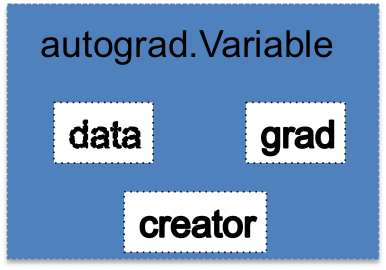
\includegraphics{../Pytorch_learning/autograd}\caption{Variable}
\end{figure}

\subsubsection{Gradients}

To calculate \textbf{gradients} from our \textit{Variable} object we apply the method \textit{<newVariable>.backward()} (where \textit{newVariable} is created from the original variable) and then extract the attribute \textit{<Variable>.grad} from the original variable. We are interested in the relation between the \textit{newVariable} and the \textit{Variable} as composition of functions, and the gradients of those functions evaluated at the a particular point. For inference it is much better to use \tif{volitile} flag when creating the variable. As we do not require backpropogation of gradients. Only the forward propagation. This is much more memory efficient. 


\subsection{Neural Networks in Torch}

Using the \textit{torch.nn} package, we can develop a NN. The \textit{torch.nn} package is dependent upon the \textit{autograd} package, to define models and differentiate them.  The \tif{nn.Module} contains layers and a method \tif{.forward(input)} returns the \tif{.output}. 

\subsubsection{Training Procedure}
\begin{enumerate}
	\item Define the NN that has some learnable parameters (or weights) 
	\item Iterate over a dataset of inputs
	\item Process input through the network
	\item Compute the loss ( how far is the output from being corrected)
	\item Propagate gradients back into the network's parameters
	\item Update the weights of the network, using a update rule
\end{enumerate} 

A simple update rule might be of the form: $weight = weight - learningRate \times gradient$. When using PyTorch, you always have to define the \tif{forward} function, but once that is done, PyTorch, using \tif{autograd}, will automatically define the \tif{backward} function.  The learnable parameters of the model can be recalled by using \textit{<class\_name\_for\_nn>.parameters()}. See \tbf{blitztor.py} for more details.\\

\tbf{Important note: } \tif{torch.nn} only supports mini-batches, the entire \tif{torch.nn} package only supports inputs that are a mini-batch of samples and not a single sample.\\

To load data in to pytorch, we load data in via an nparray and convert this array into a \textit{torch.*Tensor}.
For loading audio, use scipy and librosa. For loading text either raw Python an Cython based loading, ir NLTK and SpaCy. For vision Pytorch has the \tif{torchvision} package.  
  
 
\subsubsection{Loss function}

The loss function takes the (output, target) pairs of inputs, and computers a value that estimates how far away the output is from the target, under some measure. The Pytorch library contains many different loss functions, see documentation. See \tbf{blitzor.py} for more details.
To give all \tif{Variables} there specified gradients, up to their node in the tree, 
we simply call \tif{loss.backward()} and that accumulates all \tif{.grad}'s to calculate the gradient for the different variables, w.r.t the loss.
This also enables us to backprop the error through the network, although the existing gradients will need to be cleared. Else, you will be double adding. To zero we use the command \textit{<neural\_net\_object>.zero\_grad()}.

\subsubsection{Backprop}
To get any Variables derivative w.r.t the loss, we call, after doing \tif{loss.backward()}, \tif{<network\_name>.<Variable\_name>.\{other\_properties\}.grad}

\subsubsection{Updating the Weights}
Using the \textit{torch.optim} package we can use an array of optimizers, including SGD. See documentation. 


\end{document} 
